\documentclass[10pt,twocolumn,letterpaper]{article}

\usepackage{cvpr}
\usepackage{times}
\usepackage{epsfig}
\usepackage{graphicx}
\usepackage{amsmath}
\usepackage{amssymb}
\usepackage{CJK}
\usepackage[utf8]{inputenc}
\usepackage{listings}
\usepackage[hyphens]{url}
\usepackage{color}

\graphicspath{ {images/} }

\definecolor{dkgreen}{rgb}{0,0.6,0}
\definecolor{gray}{rgb}{0.5,0.5,0.5}
\definecolor{mauve}{rgb}{0.58,0,0.82}

\lstset{frame=tb,
  aboveskip=3mm,
  belowskip=3mm,
  showstringspaces=false,
  columns=flexible,
  basicstyle={\small\ttfamily},
  numbers=none,
  numberstyle=\tiny\color{gray},
  keywordstyle=\color{blue},
  commentstyle=\color{dkgreen},
  stringstyle=\color{mauve},
  breaklines=true,
  breakatwhitespace=true,
  tabsize=3
}


% Include other packages here, before hyperref.

% If you comment hyperref and then uncomment it, you should delete
% egpaper.aux before re-running latex.  (Or just hit 'q' on the first latex
% run, let it finish, and you should be clear).
\usepackage[breaklinks=true,bookmarks=false]{hyperref}

\cvprfinalcopy % *** Uncomment this line for the final submission

\def\cvprPaperID{****} % *** Enter the CVPR Paper ID here
\def\httilde{\mbox{\tt\raisebox{-.5ex}{\symbol{126}}}}

% Pages are numbered in submission mode, and unnumbered in camera-ready
%\ifcvprfinal\pagestyle{empty}\fi
\setcounter{page}{1}
\begin{document}
\begin{CJK}{UTF8}{gbsn}

%%%%%%%%% TITLE
\title{Project 1 MLP CNN and SNN}

\author{GIX 李心成 2016211089
% For a paper whose authors are all at the same institution,
% omit the following lines up until the closing ``}''.
% Additional authors and addresses can be added with ``\and'',
% just like the second author.
% To save space, use either the email address or home page, not both
}

\maketitle
%\thispagestyle{empty}

%%%%%%%%% ABSTRACT
\begin{abstract}
In this project, I learned Tensorflow framework, and implemented MLP, CNN and SNN with it on the MNIST data set. Finally, MLP with sigmoid activation function has the accuracy of 97.21\%, while ReLU reach the 97.87\%. CNN with traditional gradient descent algorithm has the accuracy of 99.33\%, while Adam algorithm one reach the 99.41\%. SNN has the accuracy of 90.03\%, lower than the original MLP ReLU model.
\end{abstract}

%%%%%%%%% BODY TEXT
\section{Introduction}

Project1 use the MNIST\footnote {MNIST \url{http://yann.lecun.com/exdb/mnist/}}  handwriting digits data set, to train and evaluate three neuron network models MLP, CNN and SNN separately. MNIST is a classical data set for machine learning, which contains 60,000 train images and 10,000 test images of digital handwriting. Each one is 28×28 grey image with 10 unique labels from number 0 to 9.

MLP come from the early stage of neuron network. It simplified the neuron model to a liner aggregation of previous layer input and then a activation function is used. And the BP algorithm is used to learning the weight. CNN gain a huge success these days and have a massive amount of used in a huge area of tasks in both academic and industry. It use convolution and pooling instead of the liner method in MLP, which is inspired by the mechanism in visual area of human brain. SNN is thought as the third generation of neuron network, with more inspiration of the spiking model of neurons from human brain. SNN can be super energy efficient implemented on neuromorphic hardware, with a low accuracy cost. 

In the following sections, I will introduce my method, result and discussion of three models I implemented.

\section{Method}

After some search on the Internet, I choose Tensorflow \footnote{Tensorflow \url{https://www.tensorflow.org/}} framework to do this project, for the reasons listed below:
\begin{itemize}
  \item Huge community. First I choose the language python other than the proprietary Matlab and the new comer Julia, mainly for its huge community and maturity of all the tools (Though I think Julia will be the next killer language in data Science and machine learning). And Tensorflow is the most popular among them nowadays.
  \item Supported by Google, and it targets the both side of academic and industry. 
\end{itemize}

After some struggle of picking up python3 again and learning Tensorflow,  all the method discussed below will be implemented in Tensorflow r0.11 version in python 3.5.1 environment (notice that some Tensorflow API have been changed in the newer version).

In the project folder, /summary contains the variable logs that can be visualized by Tensorboard\footnote{Tensorboard \url{https://github.com/tensorflow/tensorflow/blob/r0.11/tensorflow/tensorboard/README.md}}, use command 
\begin{lstlisting}
tensorboard --logdir="./summary"
\end{lstlisting}
and you can see the interactive graph in your browser.

\subsection{Preprocessing}

At the preprocessing stage, the input images is one channel 28*28, so the read method reshape the image to a 1D vector at the shape [784], and a batch of images with the shape [BatchSize, 784]. And the imgaes will be normolized to float type at the interval $[0.0, 1.0]$. The labels was origin a scalar denote the label 0 to 9 of the image, read method reshape the label to one hot form with the shape [10], and a batch of labels with the shape [BatchSize, 10]. 

\subsection{MLP}

Project1 appointed the structrue of MLP should used, 784-64-128-10 network and trained 30 epochs. 

The weight variables are initialized with normal distribution (stddev depends on the earch layer's units number), and bias variables are initialized with a constant slightly bigger than zero, named 0.1 in this case, for don't get two much zero gradient while training.

Two kinds of activation function have been implemented and compared, sigmoid and ReLU.

For sigmoid function, learning rate is determined at 0.3, while ReLU is 0.1. 

\subsection{CNN}

For CNN, I used ReLU activation function, trained 50 epochs at the batch size of 100. The variables are initialized almost the same as MLP. For convolution layer, I use the same convolution with stride 1 at each direction. For pooling layer, I use 2x2 average pooling. And 50\% dropout are added after each pooling.

I tried two different structures, The first one is a complex one, with structure 28x28-32c5-2s-64c5-2s-1024-10o, two hidden layer with 32 and 64 feature maps, and two full connected layer with 1024 and 10 units. The second one is a simple one, with structure 28x28-12c5-2s-64c5-2s-10o.

I use traditional gradient descent algorithm for the first complex structure, but tried two different optimize algorithm for the second simple structure, gradient descent algorithm and Adam algorithm\footnote{Adam algorithm \url{https://arxiv.org/abs/1412.6980}}. 

\subsection{SNN}

As for the SNN, I tune the MLP model with the ReLU activation function for training. I directly use the weights from the MLP, change the biases to zero for both MLP and SNN. 

SNN share the similary structure with MLP, but with some additional part. At the begining after images input, there is a spike generator. And after each layer's ReLU activation function, there is a integrate-and-fire activation function, transferring the input membrane voltage to spike generation. And at the end of softmax layer, there is a spike counter.

Spike generator use the Poisson distributed generator. If
\begin{equation}
I > \lambda * UniformRandom()
\end{equation}
which I denote for image input normalized to interval $[0.0, 1.0]$. Then a spike will be generated. I use 1.0 for parameter $\lambda$.

In integrate-and-fire activation function,
\begin{lstlisting}
V(t) = V(t - 1) + L + X(t)
If V(t) >= V_th , spike and reset V(t) = 0
If V(t) < V min, reset V(t) = V_min
\end{lstlisting}
and I set 0.0 for \texttt{V\_min}, 0.5 for \texttt{V\_th} of each layer, 0.0 for \texttt{L}.

As for spike counter, it is used to count the spike in each output class for a period of time, named 100ms as I set, to determine the final classification of a picture.

\section{Result}

\subsection{MLP}

\begin{figure}
\begin{center}
   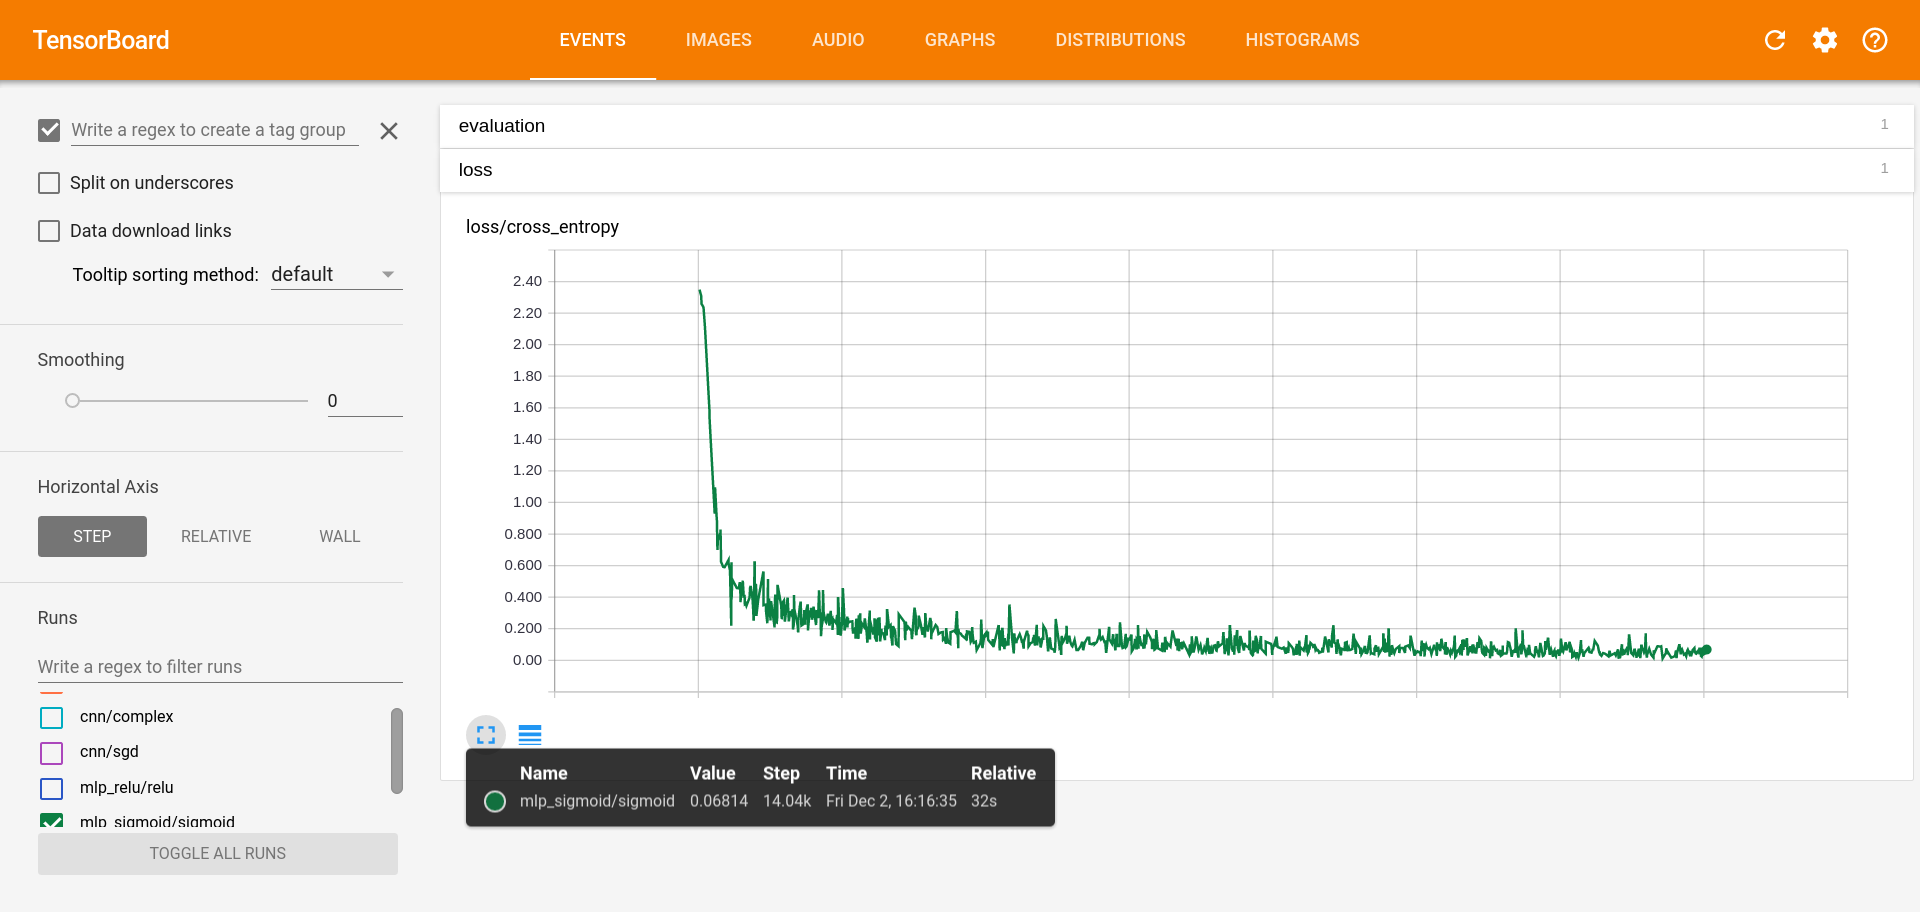
\includegraphics[width=0.9\linewidth]{mlp_sigmoid2.png}
\end{center}
\caption{Train loss of MLP sigmoid}
\label{fig:mlp_sigmoid2}
\end{figure}

\begin{figure}
\begin{center}
   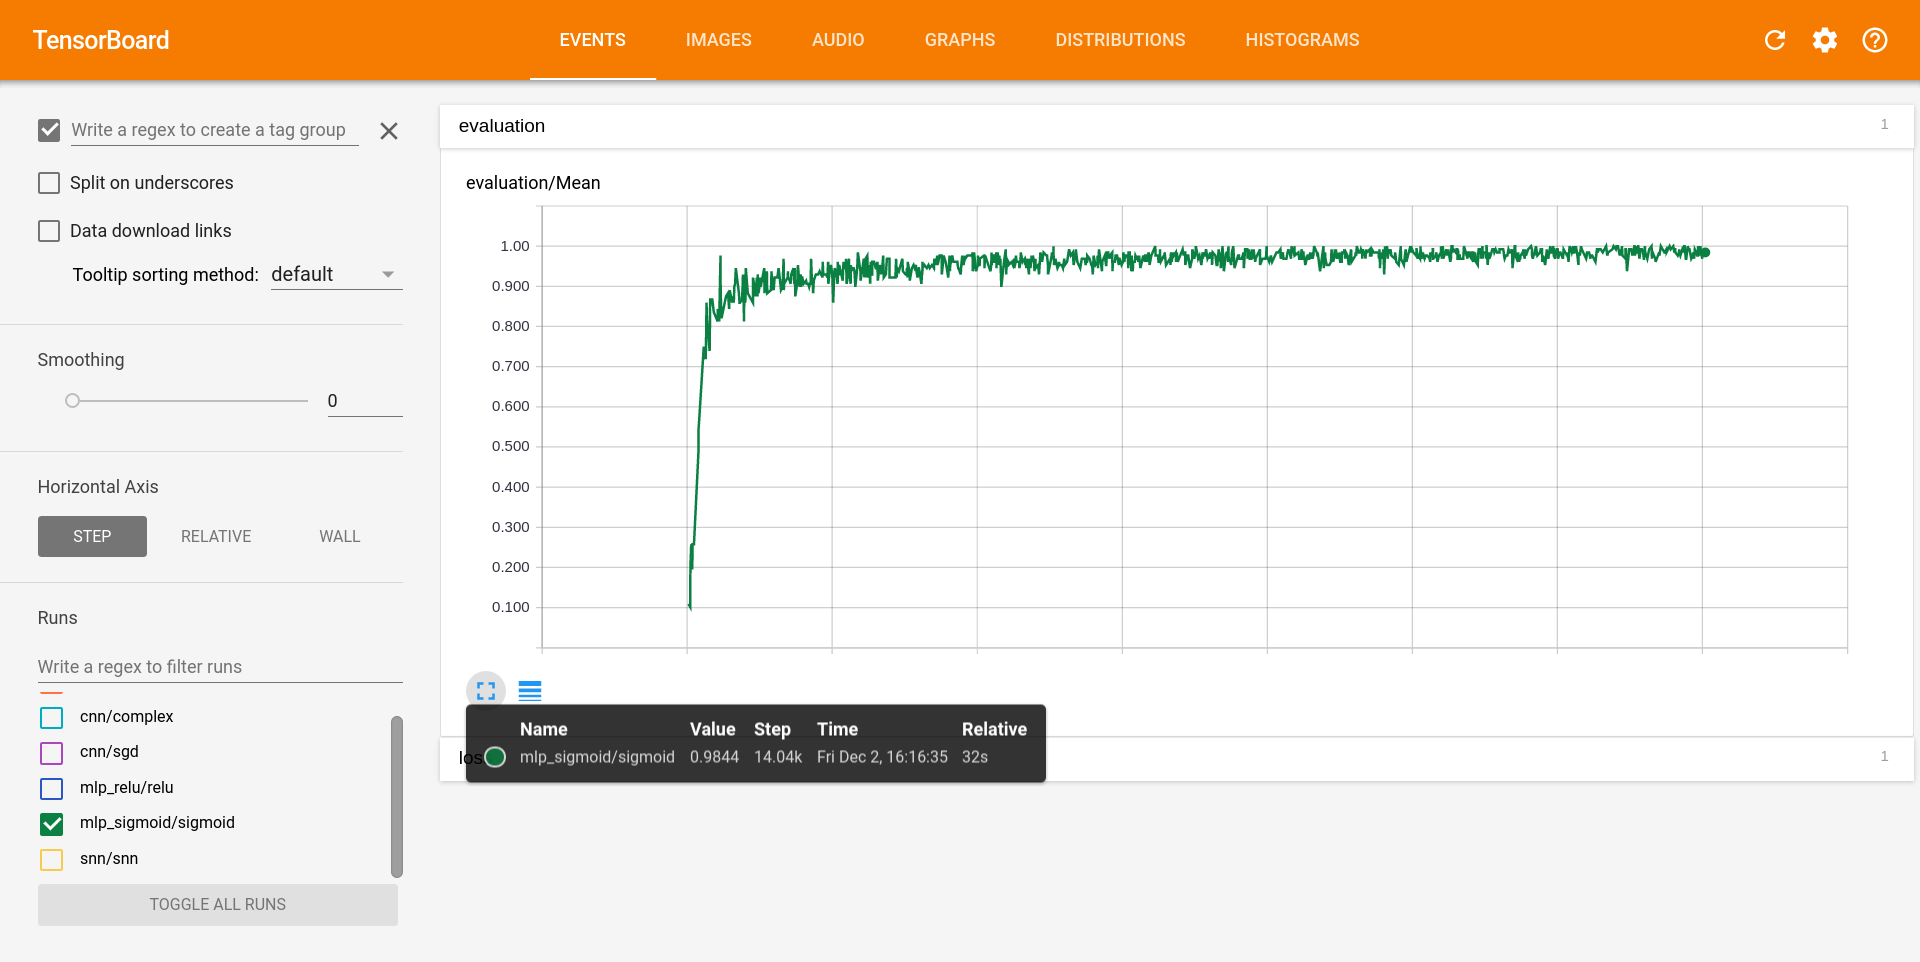
\includegraphics[width=0.9\linewidth]{mlp_sigmoid1.png}
\end{center}
\caption{Train accuracy of MLP sigmoid}
\label{fig:mlp_sigmoid1}
\end{figure}

\begin{figure}
\begin{center}
   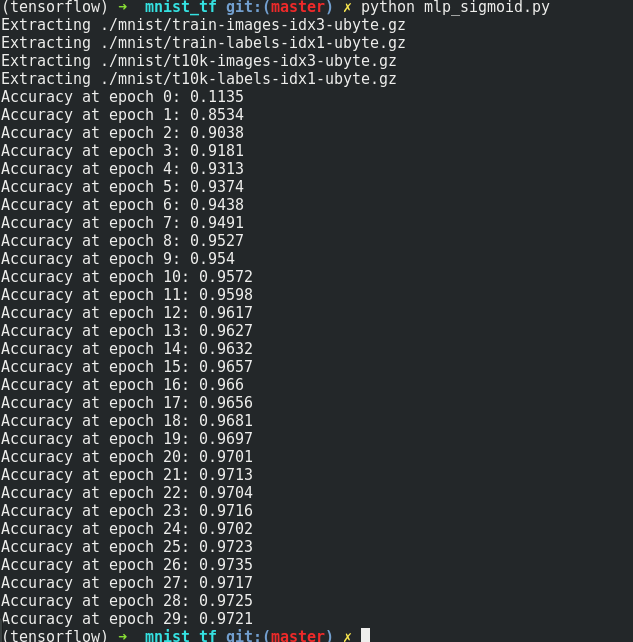
\includegraphics[width=0.9\linewidth]{mlp_sigmoid3.png}
\end{center}
\caption{Test accuracy of MLP sigmoid}
\label{fig:mlp_sigmoid3}
\end{figure}

MLP with sigmoid activation. Figure \ref{fig:mlp_sigmoid2} shows the train loss, figure \ref{fig:mlp_sigmoid1} shows the train accuracy, figure \ref{fig:mlp_sigmoid3} shows the test accuracy, with finally test accuracy 97.21\%. 

\begin{figure}
\begin{center}
   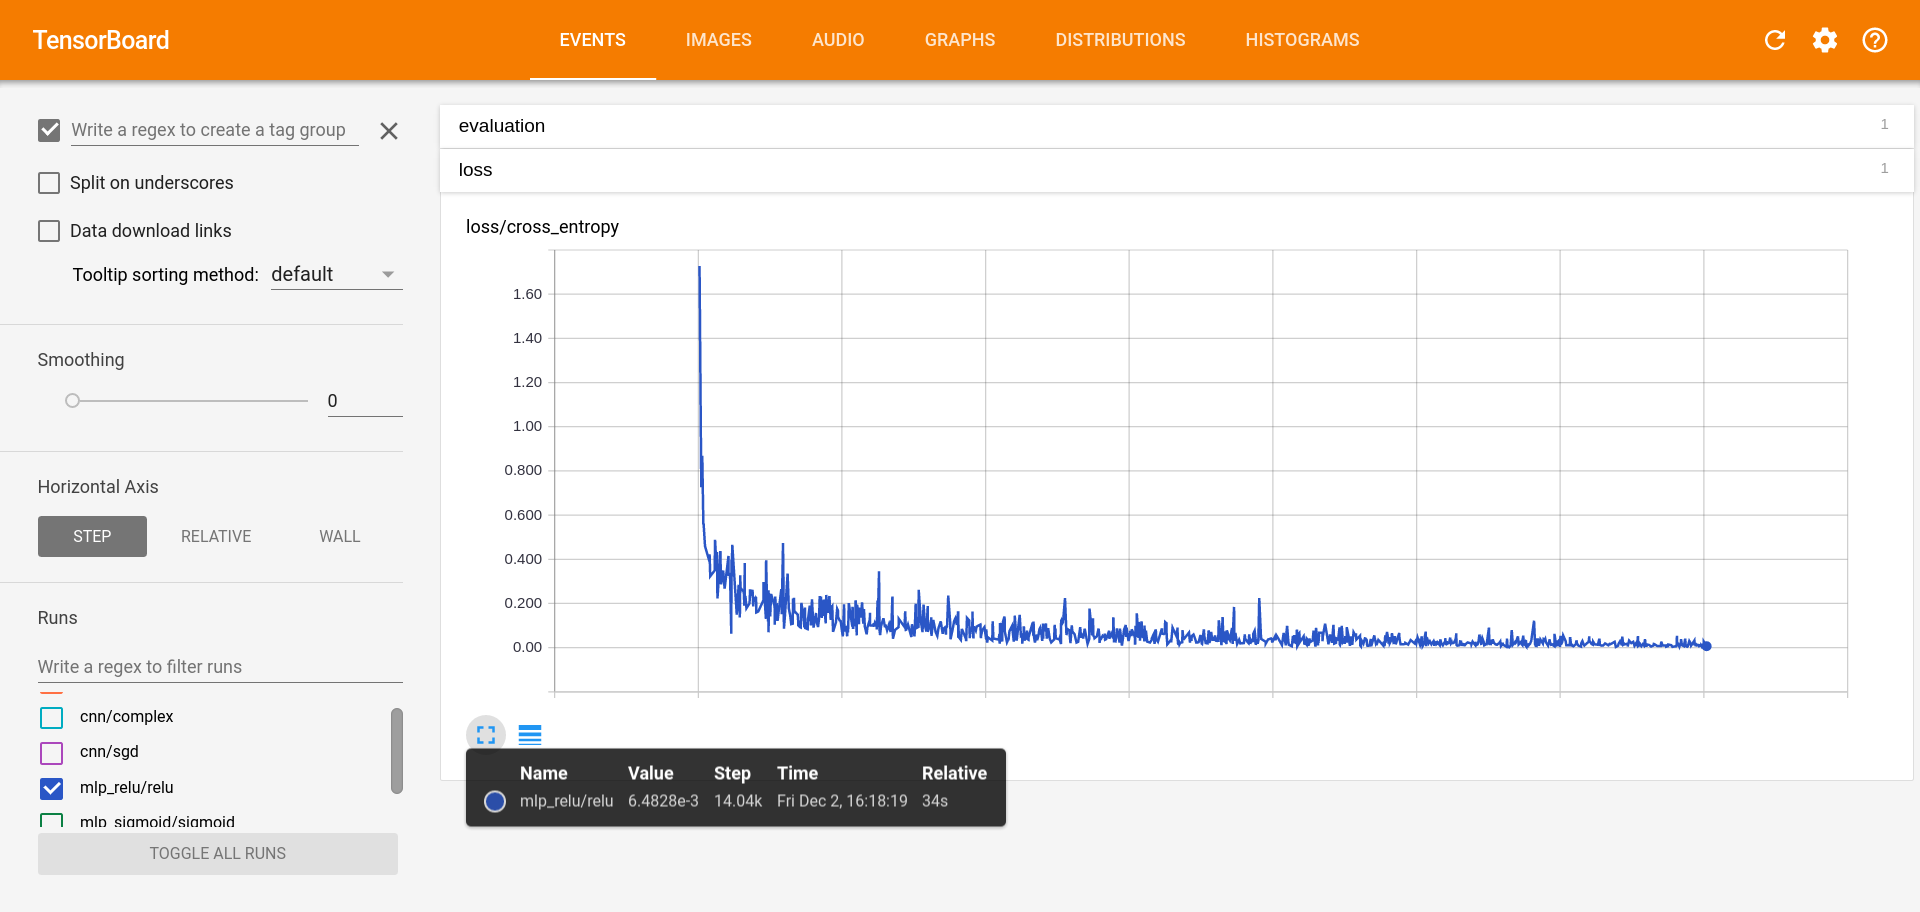
\includegraphics[width=0.9\linewidth]{mlp_relu2.png}
\end{center}
\caption{Train loss of MLP relu}
\label{fig:mlp_relu2}
\end{figure}

\begin{figure}
\begin{center}
   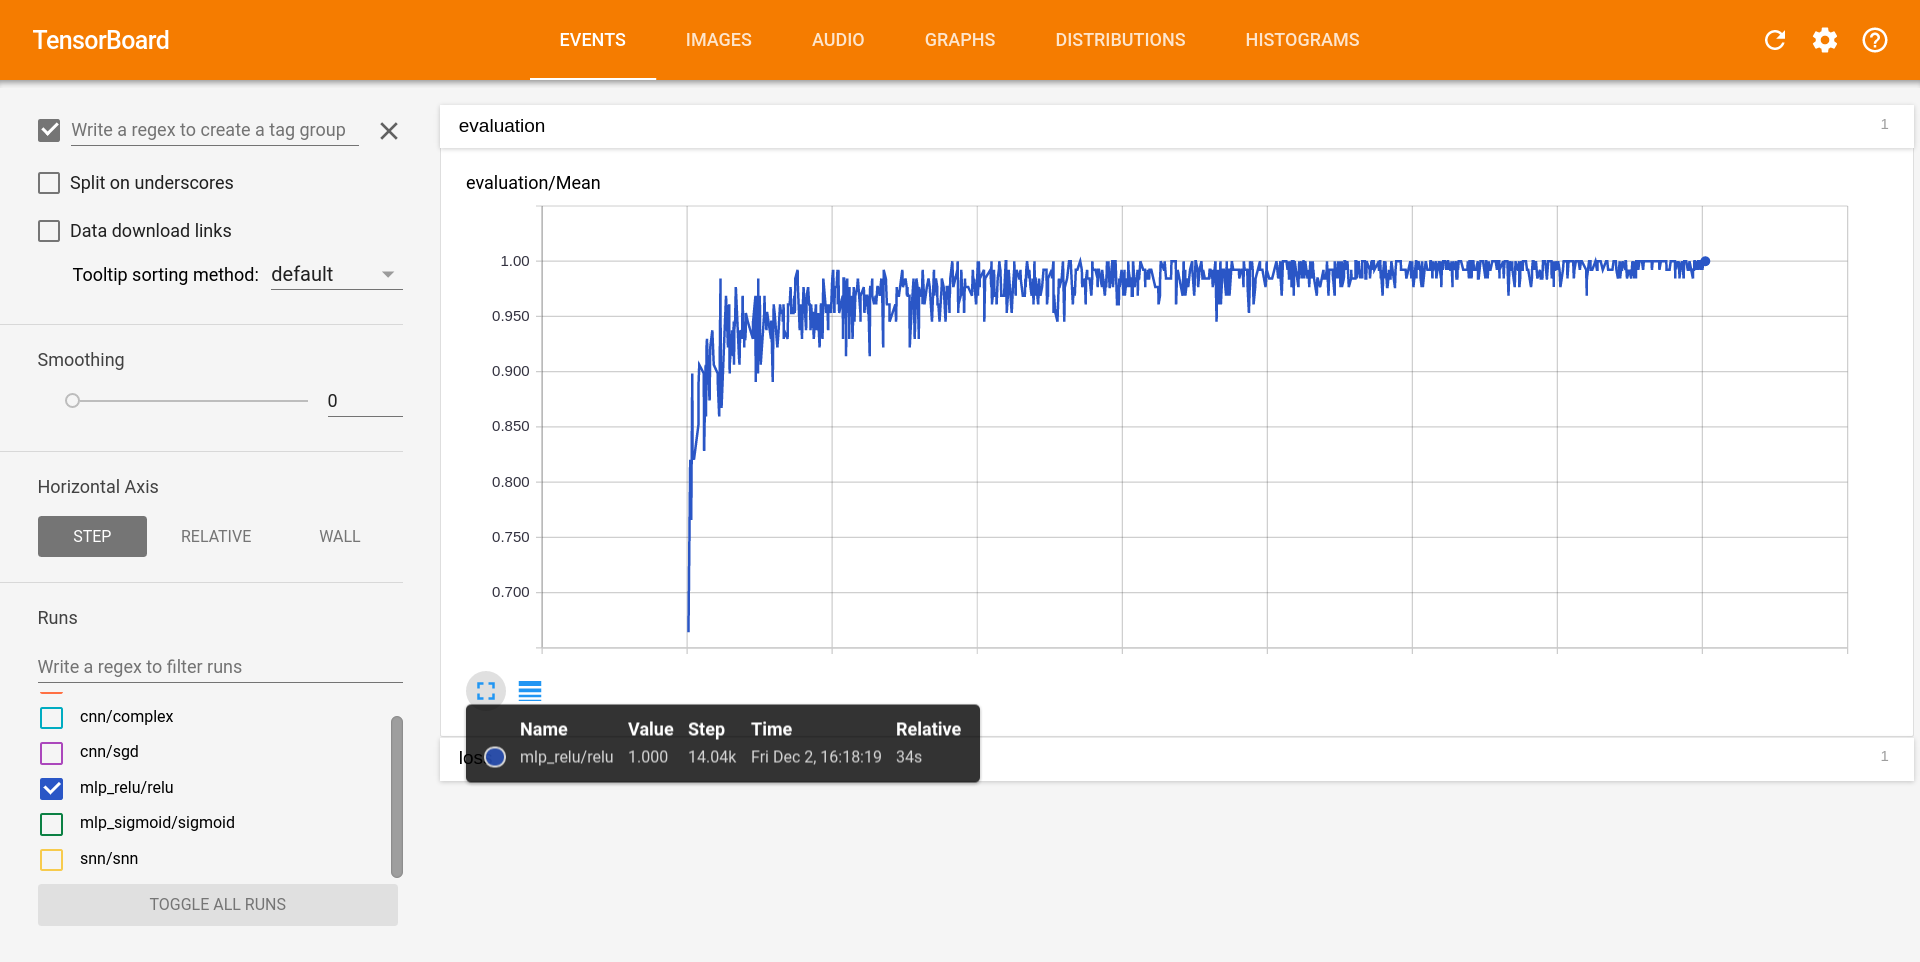
\includegraphics[width=0.9\linewidth]{mlp_relu1.png}
\end{center}
\caption{Train accuracy of MLP relu}
\label{fig:mlp_relu1}
\end{figure}

\begin{figure}
\begin{center}
   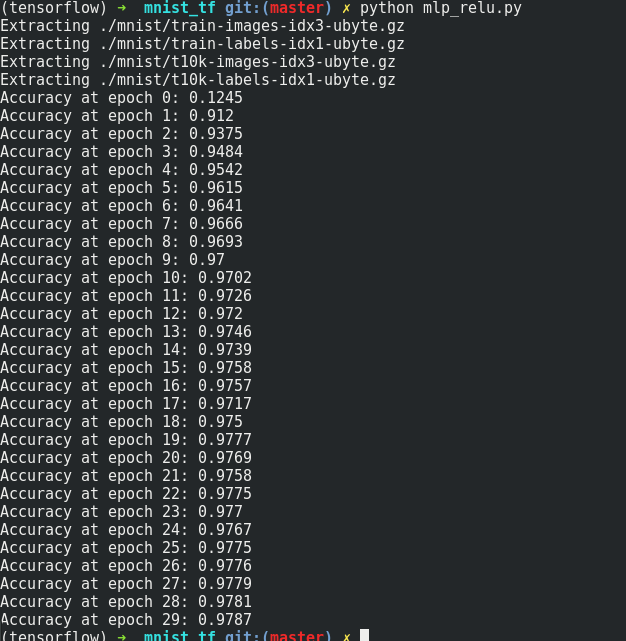
\includegraphics[width=0.9\linewidth]{mlp_relu3.png}
\end{center}
\caption{Test accuracy of MLP relu}
\label{fig:mlp_relu3}
\end{figure}

MLP with relu activation. Figure \ref{fig:mlp_relu2} shows the train loss, figure \ref{fig:mlp_relu1} shows the train accuracy, figure \ref{fig:mlp_relu3} shows the test accuracy, with finally test accuracy 97.87\%, higher than sigmoid with lesser training time. 

\subsection{CNN}

\begin{figure}
\begin{center}
   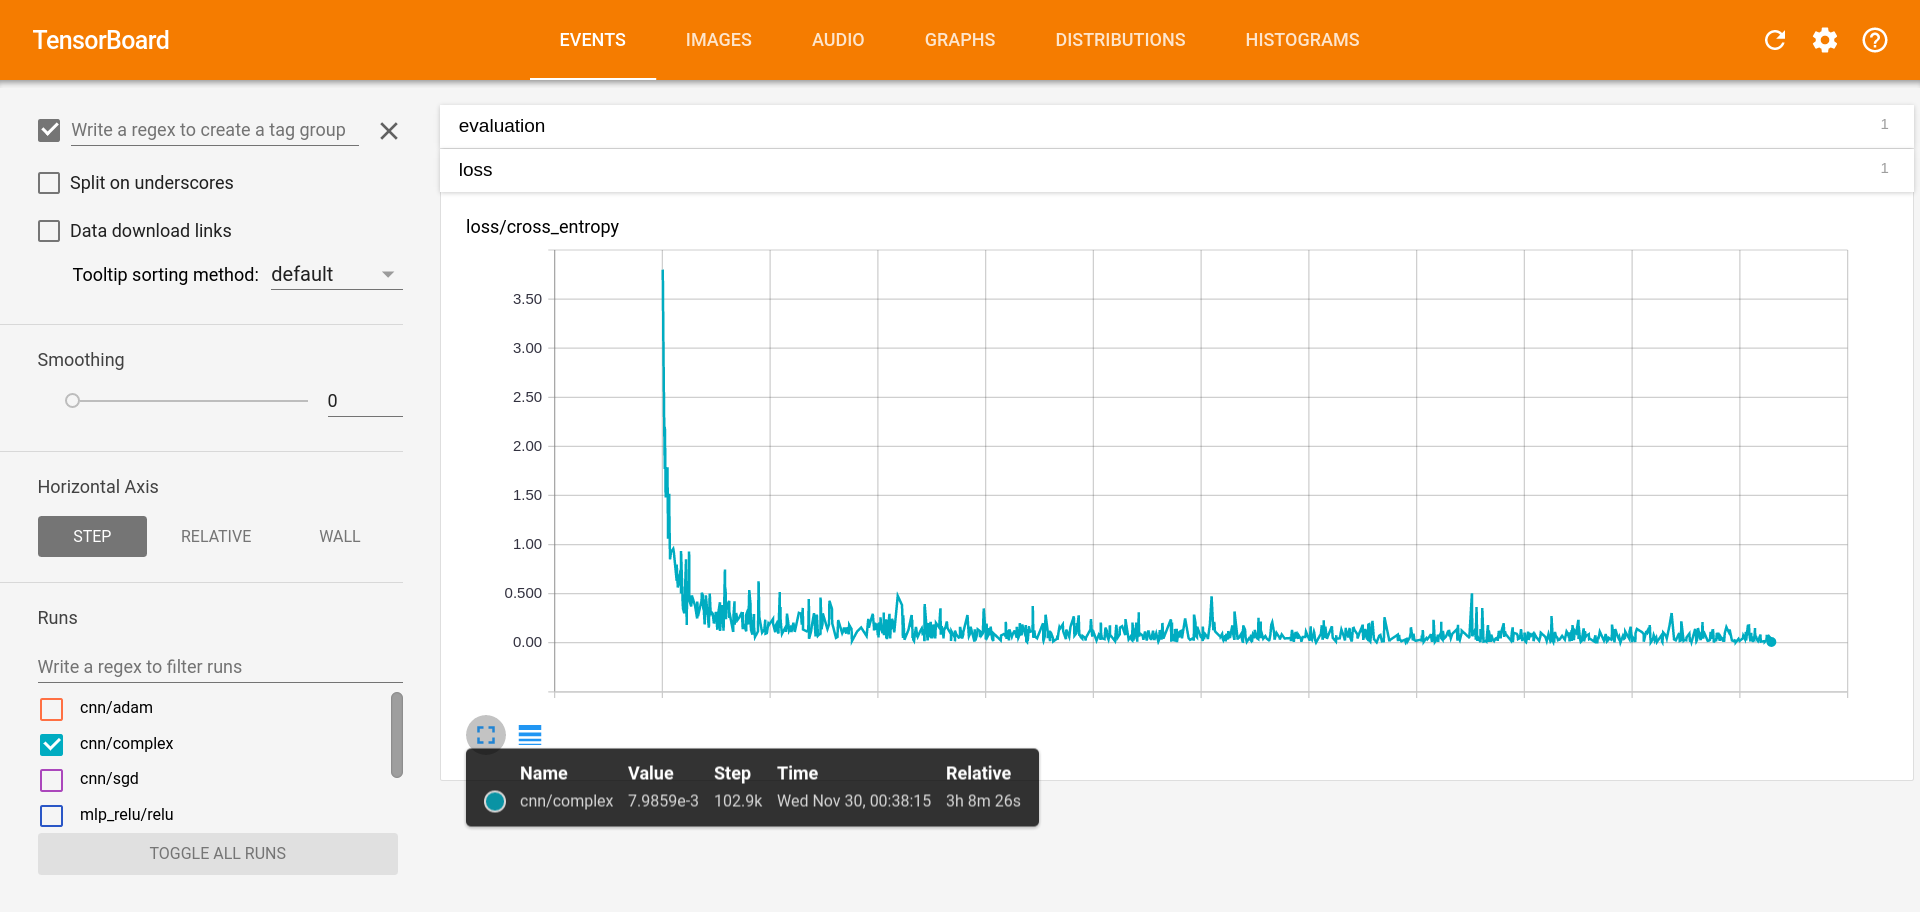
\includegraphics[width=0.9\linewidth]{cnn_complex2.png}
\end{center}
\caption{Train loss of CNN complex}
\label{fig:cnn_complex2}
\end{figure}

\begin{figure}
\begin{center}
   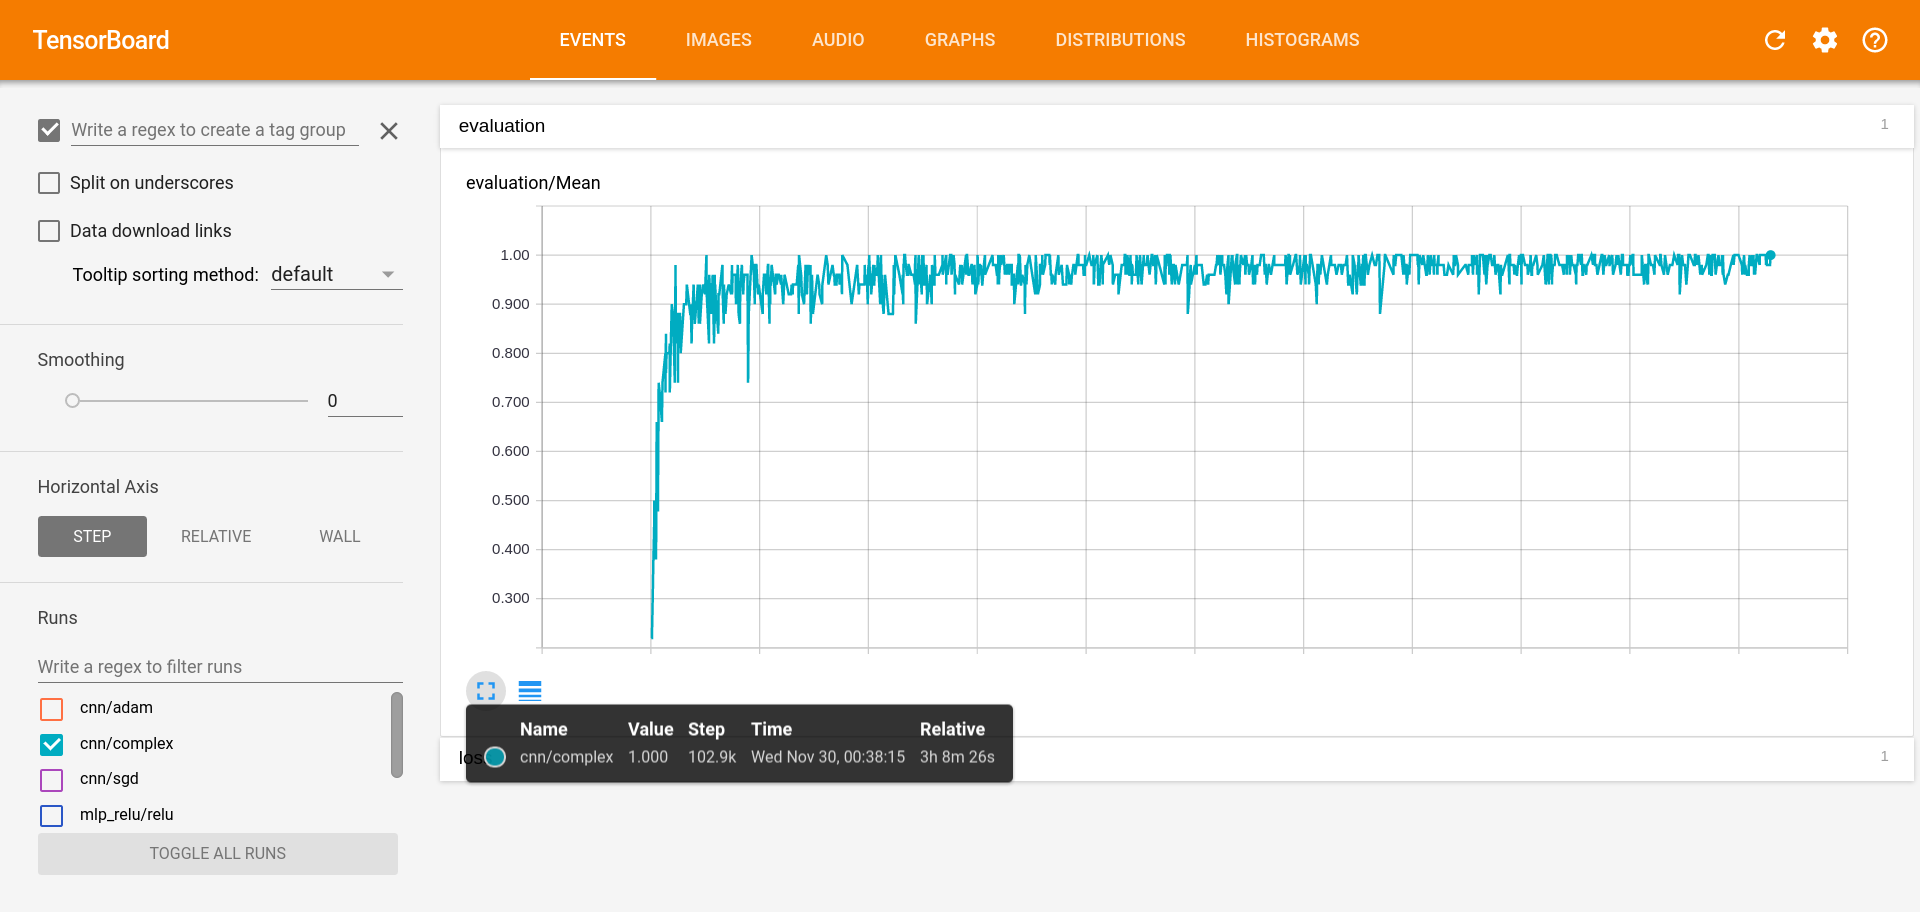
\includegraphics[width=0.9\linewidth]{cnn_complex1.png}
\end{center}
\caption{Train accuracy of CNN complex}
\label{fig:cnn_complex1}
\end{figure}

CNN with complex structure. Figure \ref{fig:cnn_complex2} shows the train loss, figure \ref{fig:cnn_complex1} shows the train accuracy. Just notice the training time, it is too long with less accuracy than the simple structure, so I give it up at early stage.

\begin{figure}
\begin{center}
   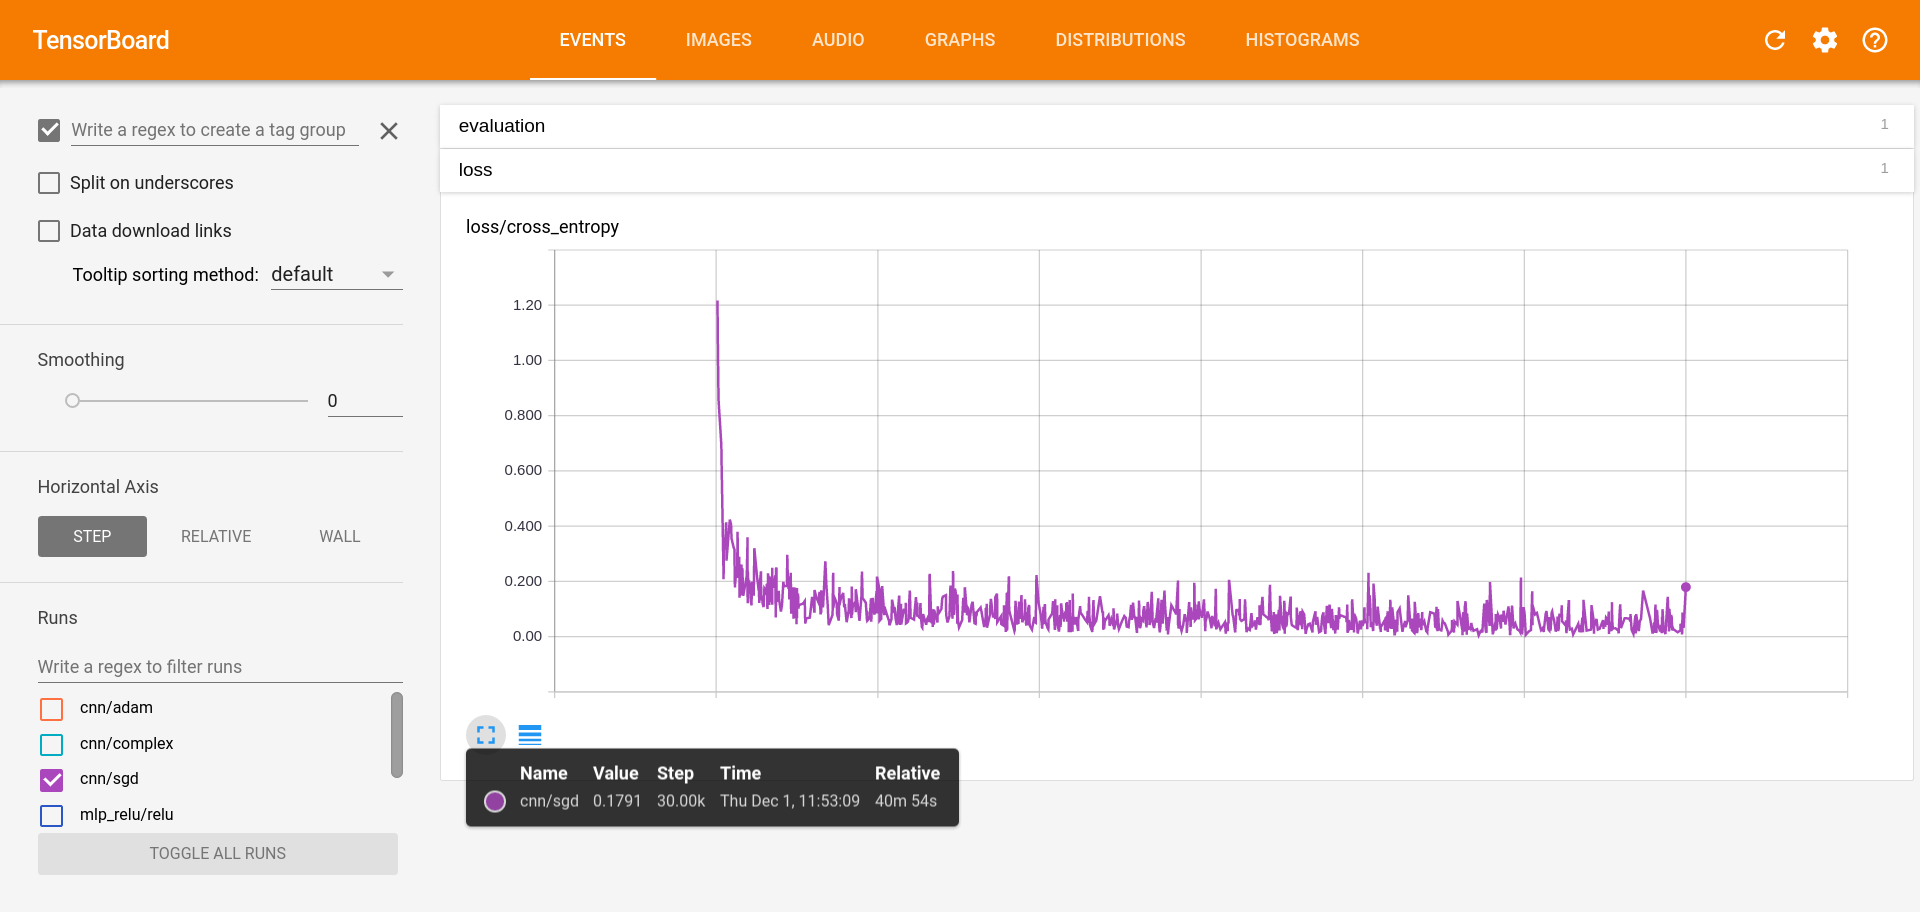
\includegraphics[width=0.9\linewidth]{cnn_sgd2.png}
\end{center}
\caption{Train loss of CNN gradient descent algorithm}
\label{fig:cnn_sgd2}
\end{figure}

\begin{figure}
\begin{center}
   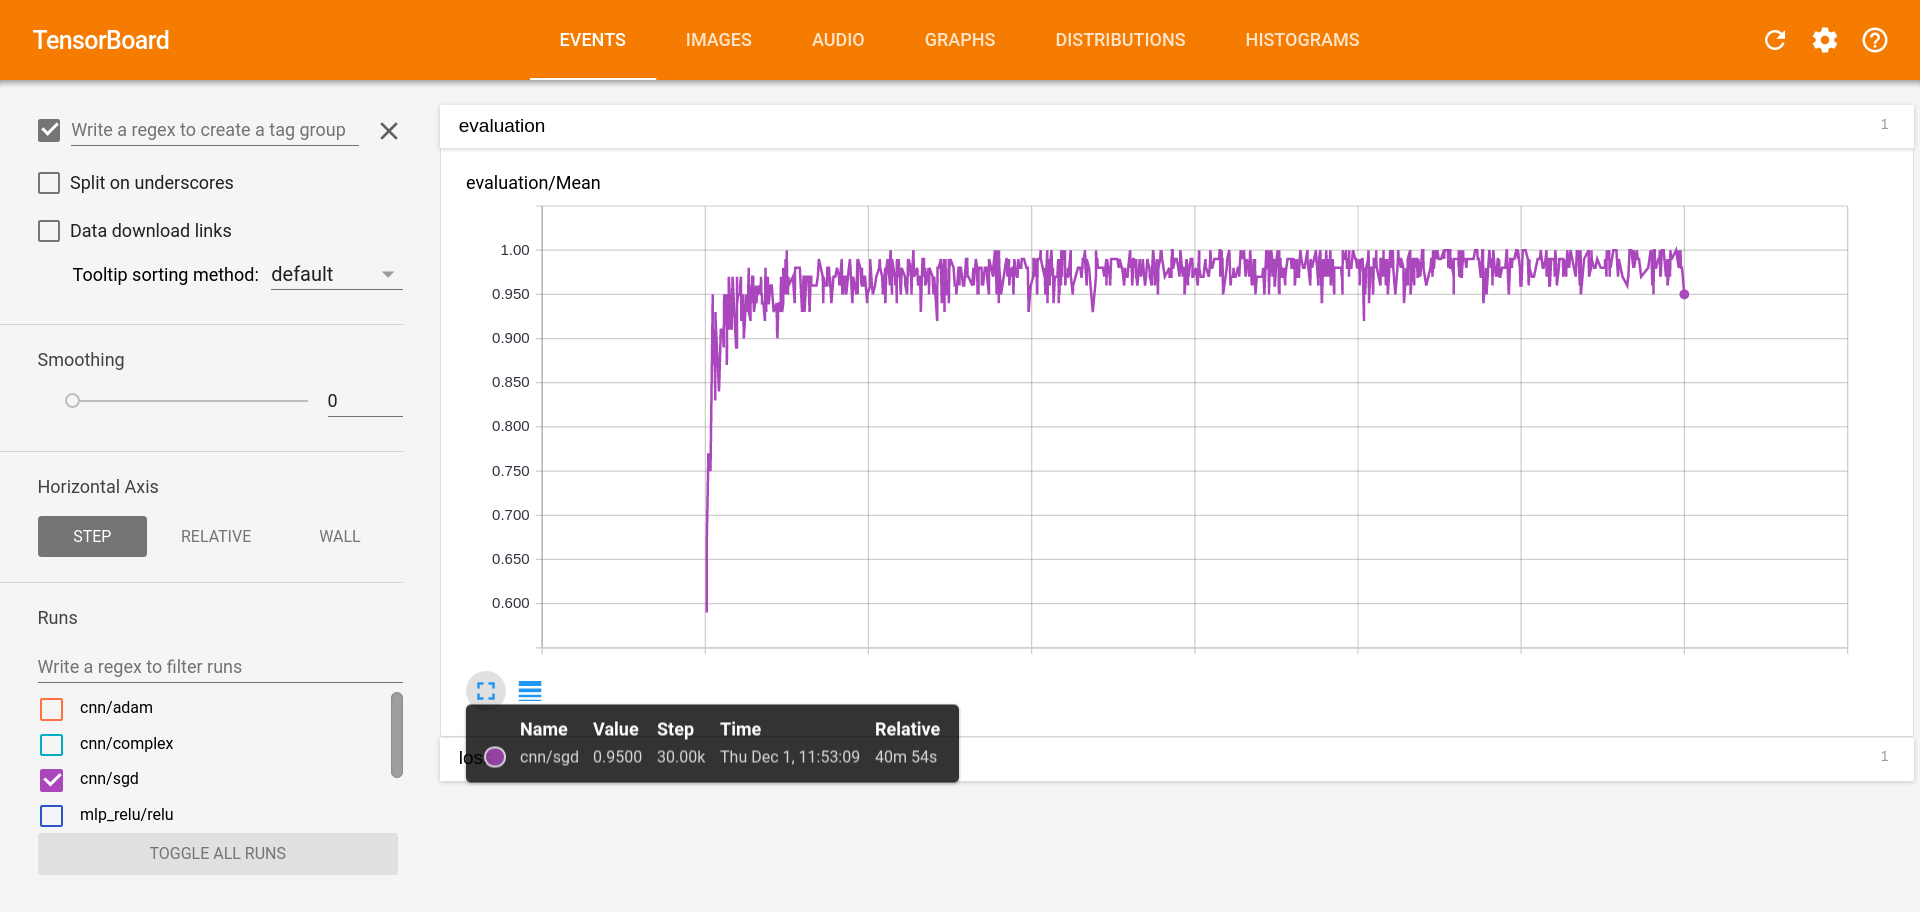
\includegraphics[width=0.9\linewidth]{cnn_sgd1.png}
\end{center}
\caption{Train accuracy of CNN gradient descent algorithm}
\label{fig:cnn_sgd1}
\end{figure}

\begin{figure}
\begin{center}
   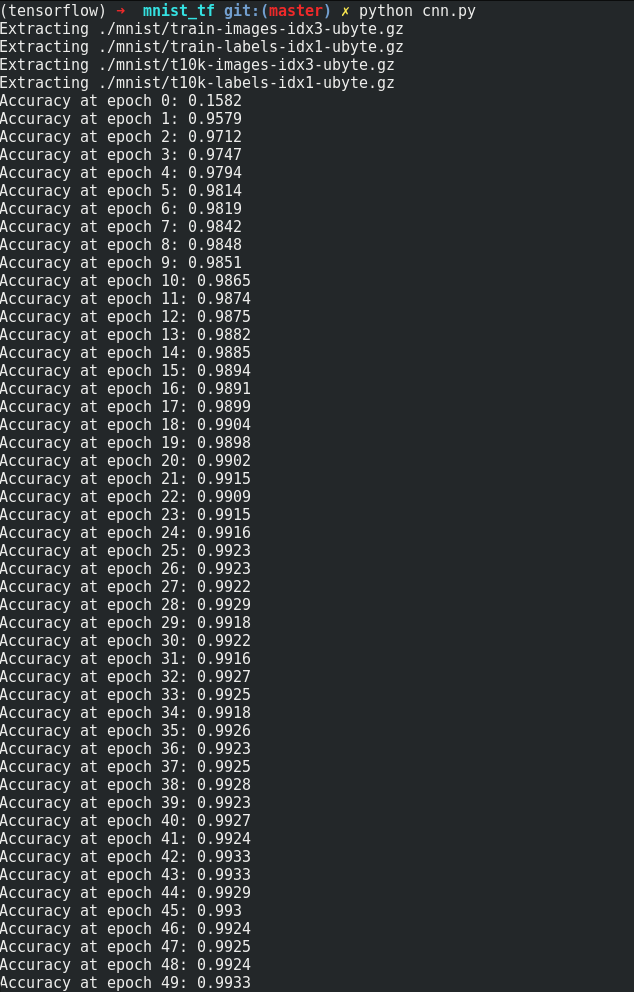
\includegraphics[width=0.9\linewidth]{cnn_sgd3.png}
\end{center}
\caption{Test accuracy of CNN gradient descent algorithm}
\label{fig:cnn_sgd3}
\end{figure}

CNN with simple structure and gradient descent algorithm. Figure \ref{fig:cnn_sgd2} shows the train loss, figure \ref{fig:cnn_sgd1} shows the train accuracy, figure \ref{fig:cnn_sgd3} shows the test accuracy, with finally test accuracy 99.33\%. Notice the training time is only 40 minutes compared to the 3 hours of the complex one.

\begin{figure}
\begin{center}
   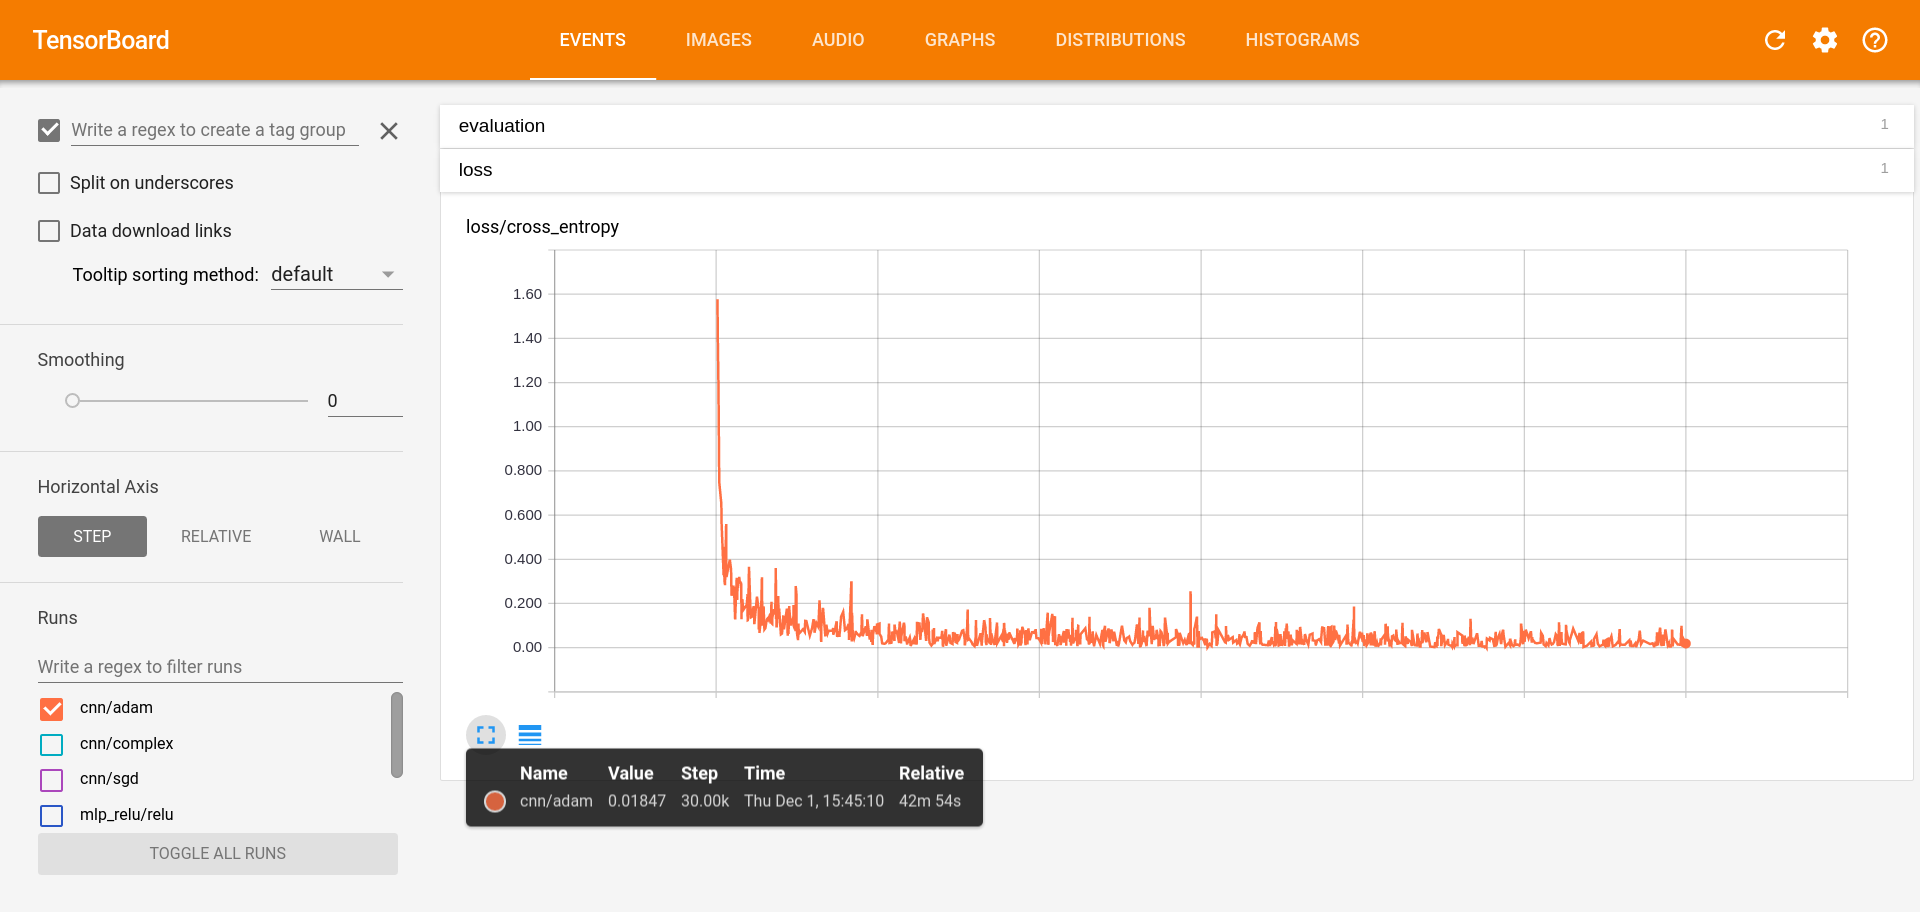
\includegraphics[width=0.9\linewidth]{cnn_adam2.png}
\end{center}
\caption{Train loss of CNN Adam algorithm}
\label{fig:cnn_adam2}
\end{figure}

\begin{figure}
\begin{center}
   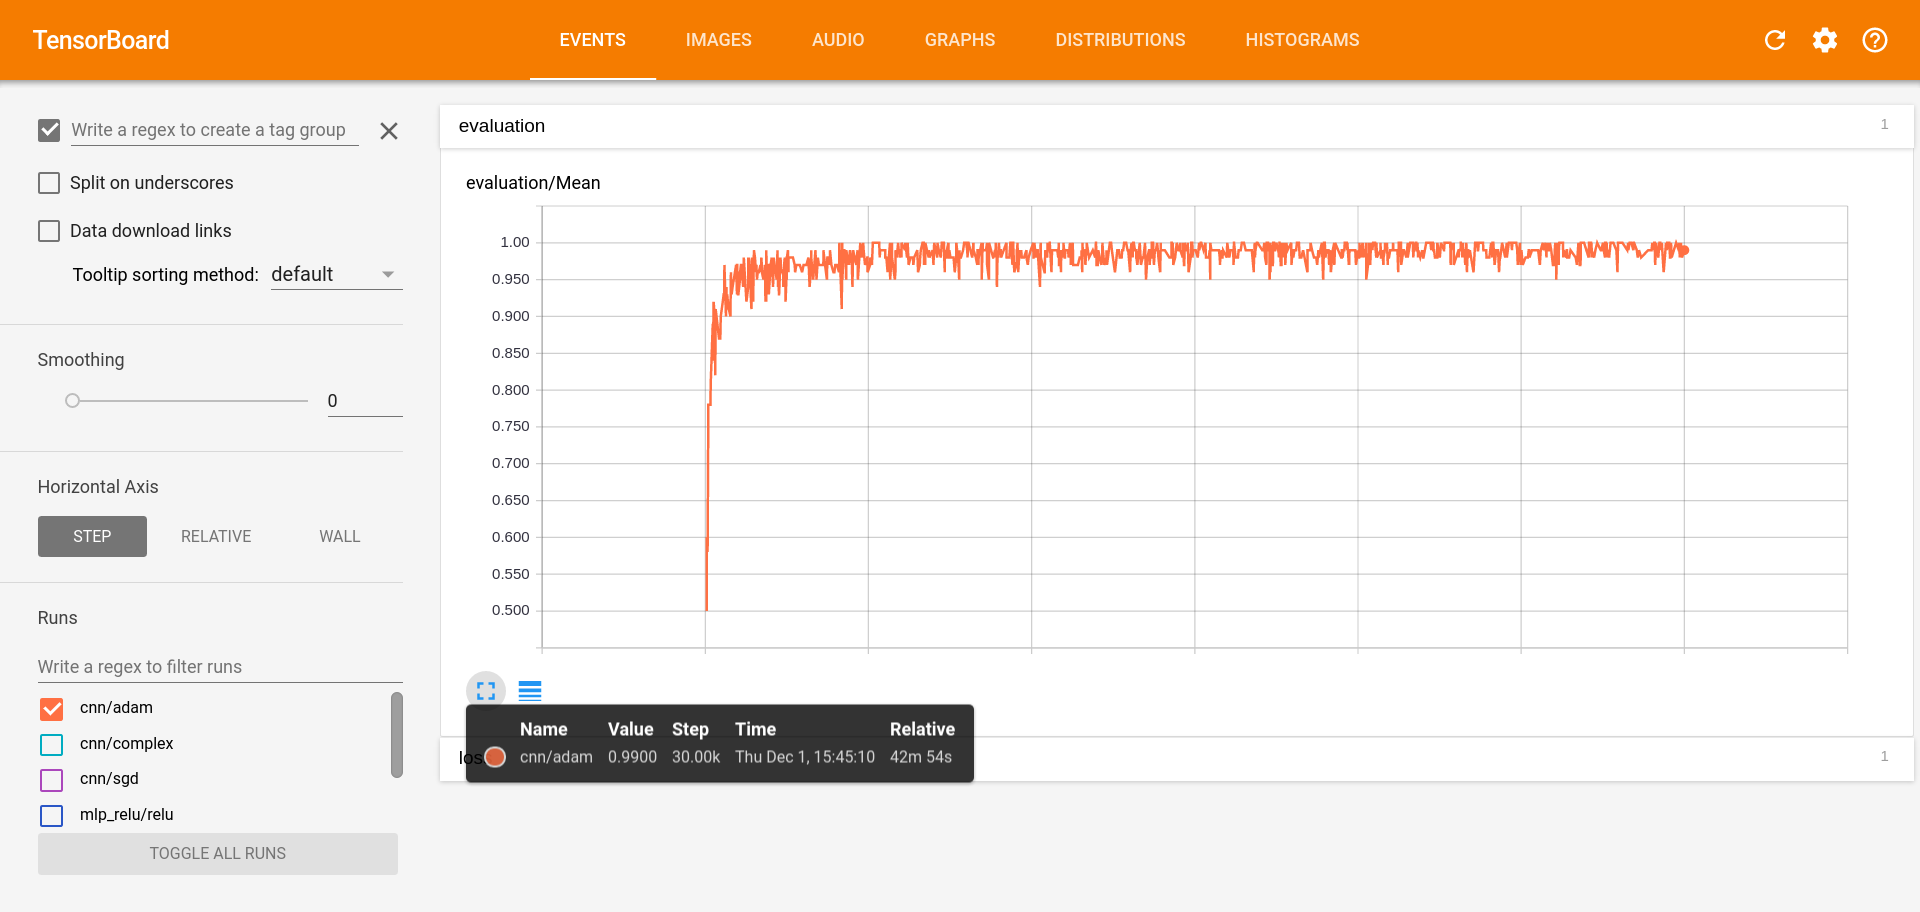
\includegraphics[width=0.9\linewidth]{cnn_adam1.png}
\end{center}
\caption{Train accuracy of CNN Adam algorithm}
\label{fig:cnn_adam1}
\end{figure}

\begin{figure}
\begin{center}
   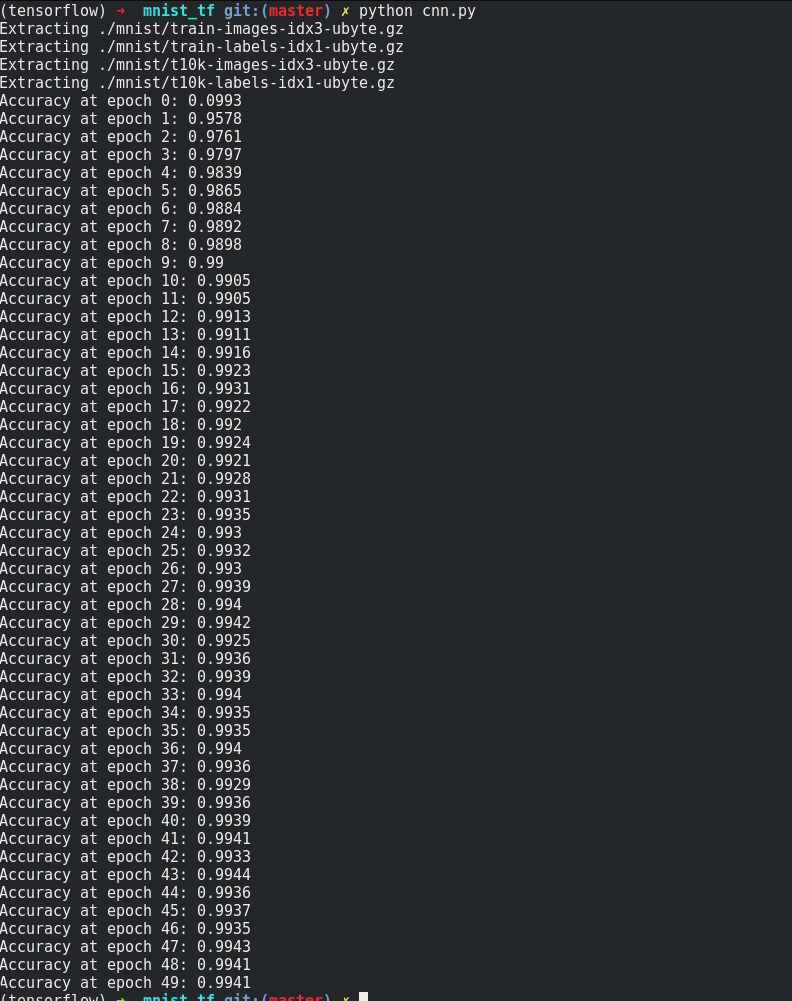
\includegraphics[width=0.9\linewidth]{cnn_adam3.png}
\end{center}
\caption{Test accuracy of CNN Adam algorithm}
\label{fig:cnn_adam3}
\end{figure}

CNN with simple structure and gradient descent algorithm. Figure \ref{fig:cnn_adam2} shows the train loss, figure \ref{fig:cnn_adam1} shows the train accuracy, figure \ref{fig:cnn_adam3} shows the test accuracy, with finally test accuracy 99.41\%, a little higher than traditional gradient descent algorithm.

\subsection{SNN}

\begin{figure}
\begin{center}
   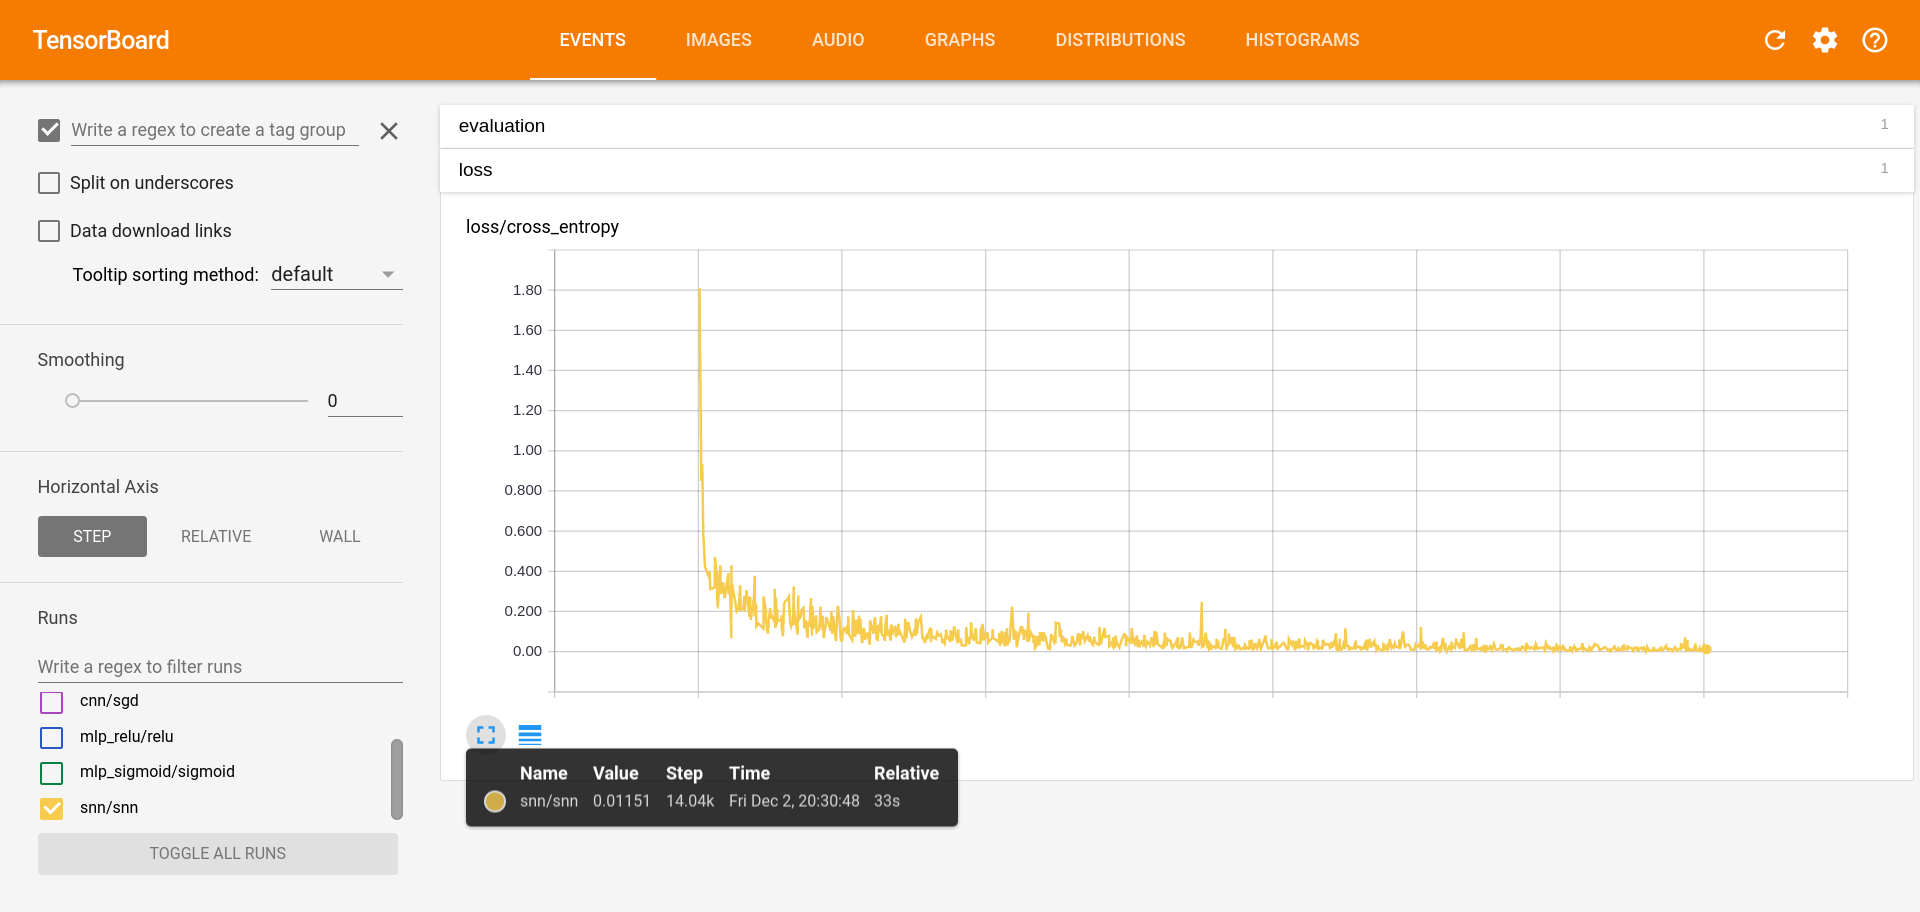
\includegraphics[width=0.9\linewidth]{snn2.png}
\end{center}
\caption{Train loss of SNN}
\label{fig:snn2}
\end{figure}

\begin{figure}
\begin{center}
   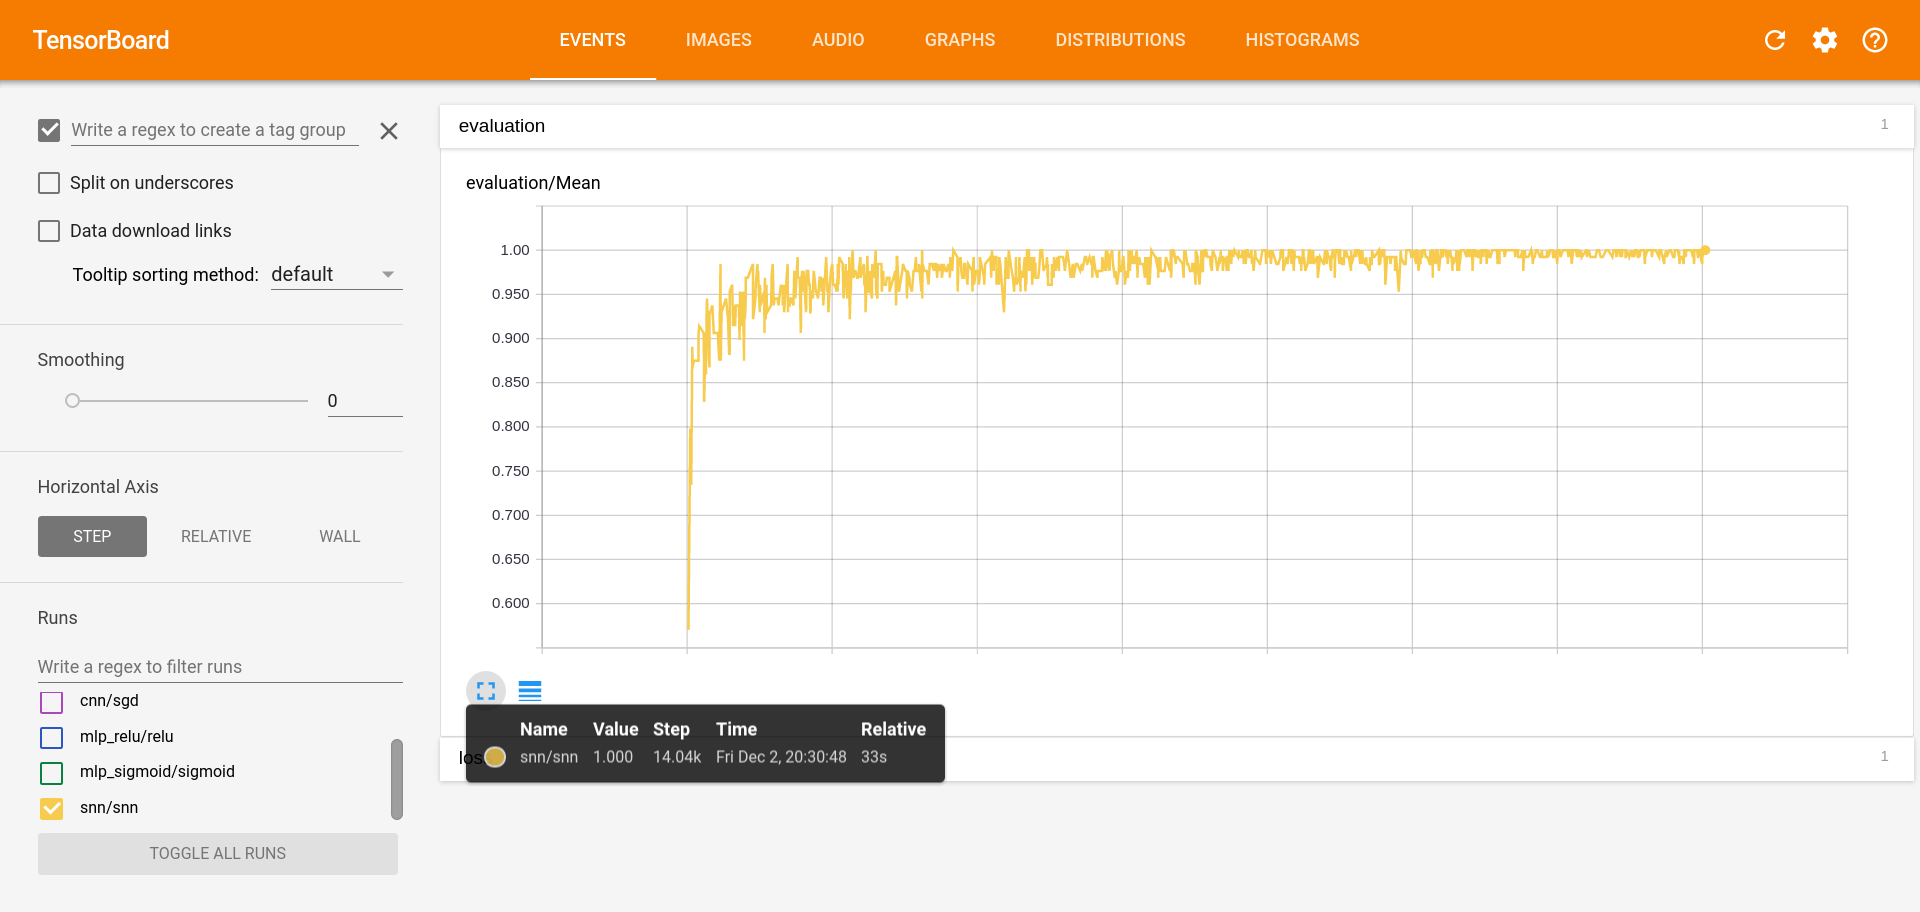
\includegraphics[width=0.9\linewidth]{snn1.png}
\end{center}
\caption{Train accuracy of SNN}
\label{fig:snn1}
\end{figure}

\begin{figure}
\begin{center}
   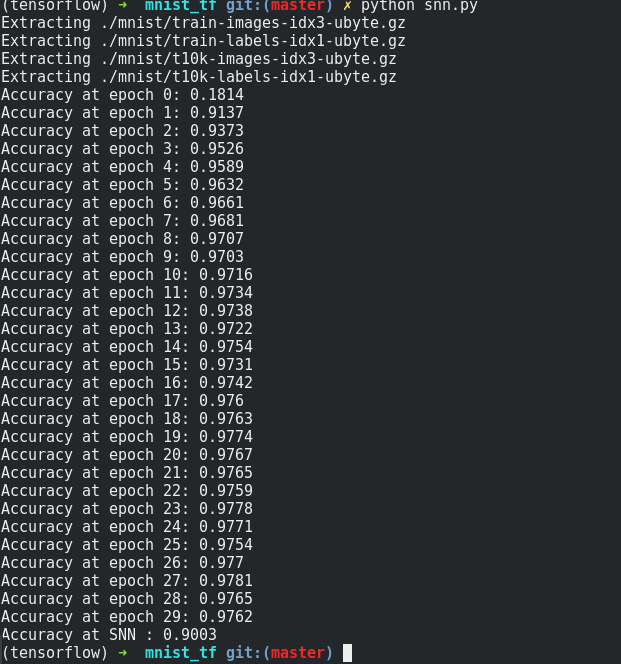
\includegraphics[width=0.9\linewidth]{snn3.png}
\end{center}
\caption{Test accuracy of SNN}
\label{fig:snn3}
\end{figure}

SNN figures. Figure \ref{fig:snn2} shows the train loss, figure \ref{fig:snn1} shows the train accuracy, almost the same as MLP with ReLU activation function. Figure \ref{fig:snn3} shows the test accuracy, with finally test accuracy 90.03\%, lower than original MLP solution.

\section{Discussion}

\subsection{MLP}

The weight variables are initialized with normal distribution and bias variables are initialized with a constant slightly bigger than zero is effective for not get two much zero gradient while training.

After some trial, learning rate is determined at 0.3 for sigmoid, while ReLU is 0.1. If learning rate is larger than that, such as 1.0 I've tried, then the loss will go down very fast at first, but will easily overfit after several epochs, which cause a low accuracy finally. And if learning rate is smaller than that, loss will go down too slow and not sufficiently learned. Because of the ReLU will converge faster than sigmoid, so the learning rate is little smaller.

\subsection{CNN}

Add 50\% dropout after each pooling layer lower the training time while decrease the overfit chances tremendously.

As the result show, the complex structure have a much logner training time, but with limited gain. As I am considered, it is mainly caused by the simplicity of the MNIST data set. Digital handwriting image has relatively less features than normal colorful daily images, so simple structure is enough for the task.

Adam algorithm add some advanced features to traditional gradient descent algorithm, such as stochastic descent, adaptive estimates of lower-order momentum. Which means it have a bigger step at the beginning and lower step at the end. It converges faster than traditional gradient descent but have higher accuracy finally.

\subsection{SNN}

To achieve the minimal accuracy loss, there are some tricks.

Use the ReLU as the activation function, because ReLU can prevent the merge of negative number.

Set the biases to zero so that the spike can be controlled.

Choose the right threshold voltage of each layer. This is the most critical part to have a decent loss of accuracy. When threshold is too high, too little spikes are generated. When threshold is too low, too many spikes are generated. Both will cause SNN have no ability to distinguish the images. Or otherwise you can do the weight normalization, which may gain a better result than manually trial.

%-------------------------------------------------------------------------
\end{CJK}
\end{document}
